\section{Comparison}
	\label{sec:comparison}
	In order to assert that one optimisation technique is superior to another, we will need to employ some degree of statistical analysis. This is because, among other reasons, all of the optimisation techniques concerned are non-deterministic. This means that on individual runs each optimisation technique may yield vastly different results. Some of these may be superior to others more often than not and so we quantify this in order to be more certain. See page over.
	\subsection{Improvement Performance Profiles}
		\label{sec:comparison_improvement_profile} 
		To graphically demonstrate the performance of the optimisers against each other, we recorded their best found result at each step of the iteration with the environment variables. Some translation was done for comparison of results where there was not a strict relationship between an iteration and objective function calls.
		\begin{figure}[H]
		\centering
		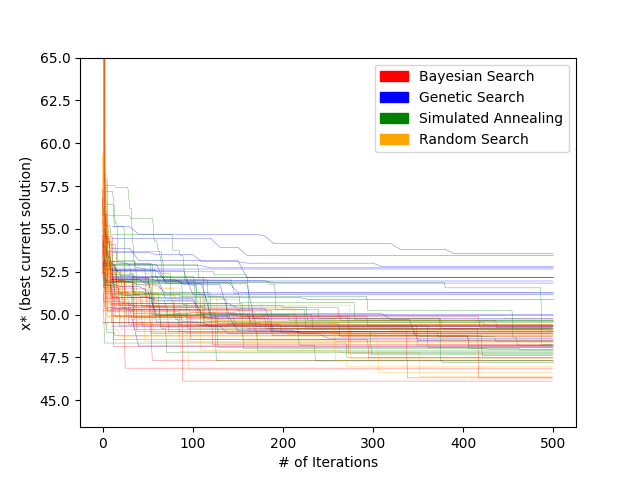
\includegraphics[scale=0.75]{graphics/performance}
		\caption{Performance of Bayesian Search, Genetic Search, Simulated Annealing and Random Search compared over 25 runs of 500 iterations.}
		\end{figure}
	\subsection{Mann-Whitney U Test}  
		\label{sec:comparison_mann-whitney} 
		The Mann-Whitney U test is a test of the null hypothesis that for a random selection of values (A and B) from two discrete populations, the likelihood of A being greater than B is equal to B being greater than A. This test produces a `U statistic' from the following formula:
		\begin{equation}
			U = \sum\limits_{i=1}^n\sum\limits_{j=1}^m S(A_i, B_j)
		\end{equation}
		S is as follows:
		\begin{equation}
			S(A, B) = 
			\begin{cases}
				1, \:if\: B < A, \\
				\frac{1}{2}, \:if\: B = A, \\
				0, \:if\: B > A.
			\end{cases}
		\end{equation}
		From this test, we can extract a $\rho$ statistic by dividing U by the maximum possible value of U ($n \times m$). This is done for each test carried out in the table below. For all results, $n = m = 25$. \\
		\begin{center}
			\small
			% \begin{longtable}{| p{2cm} | p{2cm} | p{2cm} | p{2cm} | p{2cm}|}
			% 	\hline
			% 	 \diagbox[innerwidth=2cm,height=1.5cm]{B}{A} & \textbf{Bayesian Search} & \textbf{Genetic Search} & \textbf{Simulated Annealing} & \textbf{Random Search} \\
			% 	\hline
			% 	\textbf{Bayesian Search} & N/A & U = 75, \newline $\rho$ = 0.1200 & U = 280, \newline $\rho$ = 0.4480 & U = 278, \newline $\rho$ = 0.4448 \\
			% 	\hline
			% 	\textbf{Genetic Search} & U = 550, \newline $\rho$ = 0.8800 & N/A & U = 545, \newline $\rho$ = 0.8720 & U = 538, \newline $\rho$ = 0.8608 \\
			% 	\hline
			% 	\textbf{Simulated Annealing} & U = 345, \newline $\rho$ = 0.5520 & U = 80, \newline $\rho$ = 0.1280 & N/A & U = 304, \newline $\rho$ = 0.4864 \\
			% 	\hline
			% 	\textbf{Random Search} & U = 347, \newline $\rho$ = 0.5552 & U = 87, \newline $\rho$ = 0.1392 & U = 321, \newline $\rho$ = 0.5136 & N/A\\
			% 	\hline
			% \end{longtable}
		\end{center}
	\subsection{Takeaways} 
		\label{sec:comparison_takeaways} 
		From our performance profiles and Mann-Whitney U test tables it is clear that while Bayesian Search is superior to the traditional methods we have considered, the difference is not significantly vast for the environment as defined in appendix \ref{app:bounds}. In environments with a larger number of decision variables and a significantly more expensive objective function, I believe that this difference would be even more pronounced.
		